\documentclass[conference]{IEEEtran}

\usepackage{cite}
\usepackage{amsmath,amssymb}
\usepackage{booktabs}
\usepackage{array}
\usepackage{tabularx}
\usepackage{url}
\usepackage{graphicx}
\usepackage{float}
\usepackage{placeins}
\usepackage{xcolor}

\newcommand{\chg}[1]{{\color{blue}#1}}

\setlength{\textfloatsep}{4pt plus 1.0pt minus 1.0pt}
\setlength{\floatsep}{3pt plus 1.0pt minus 1.0pt}
\setlength{\intextsep}{3pt plus 1.0pt minus 1.0pt}
\setlength{\abovecaptionskip}{2pt}
\setlength{\belowcaptionskip}{2pt}

\title{Phoenix: Deterministic Self-Healing and Fault Tolerance for Autonomous Desktop Automation}

\author{
\IEEEauthorblockN{
Ramani G\textsuperscript{1},
Akshitha V G\textsuperscript{2},
Kruthin Shanmuk Yadav CG\textsuperscript{3},
Dhanyashree G V\textsuperscript{4},
Kaushal K\textsuperscript{5}
}
\IEEEauthorblockA{
Department of Computer Science and Engineering (AI \& ML)\\
AMC Engineering College, Bengaluru, Karnataka, India\\
Emails: gowrisan.ramani@amceducation.in, akshithavg1@gmail.com, \\
kruthin008@gmail.com, dhanyashreegv206@gmail.com, kaushalk123000@gmail.com
}
}

\begin{document}

\maketitle

\begin{abstract}
Reliable execution in multi-agent desktop automation requires robust error mitigation beyond raw task scheduling. Real-world automation workflows routinely encounter application crashes, missing file dependencies, transient network timeouts, and state inconsistencies. Existing AI agent recovery approaches rely heavily on continuous model-based replanning. These methods can introduce additional inference latency, token usage, and variability in recovery behavior. In this paper, we present the self-healing subsystem of Phoenix Agents, a deterministic, bounded recovery framework designed to diagnose and remediate execution exceptions in multi-agent desktop workflows without requiring an active Large Language Model (LLM) during the recovery loop. The recovery mechanism is structured into five distinct operational stages: error parsing, root-cause classification, strategy selection, patch generation, and retry execution. Recovery decisions follow typed contract assertions, deterministic rules, and a fixed retry budget ($K_{\text{max}} = 3$). Empirical evaluation across 125 controlled fault-injection trials demonstrates that \chg{on 125 injected faults, the pipeline recovered all 75 faults in the three recoverable classes (Missing Resource, Timeout, Tool/Adapter Failure; 75/75) and rejected all 50 faults in the two unsafe classes (Invalid Action, State Inconsistency; 50/50), giving 60.0\% overall recovery (75/125) once rejections are counted, with a mean software-level recovery latency of 1.30~ms.} Controlled comparisons show a workflow completion rate of 100\% with deterministic recovery enabled versus 0\% with recovery disabled under transient faults.
\end{abstract}

\begin{IEEEkeywords}
Phoenix Agents, Self-Healing, Multi-Agent Systems, Desktop Automation, Fault Recovery, Deterministic Recovery, Error Mitigation.
\end{IEEEkeywords}

\section{Introduction}
Multi-agent desktop and browser automation frameworks orchestrate complex workflows across web browsers, native applications, operating system terminals, and local file systems~\cite{bajoria2026}. However, executing tasks across heterogeneous host environments inherently exposes software agents to dynamic execution failures, such as transient network timeouts, missing file dependencies, altered DOM locators, process crashes, and permission denials.

In conventional script-based automation systems (e.g., Selenium, AutoHotkey), a single runtime exception causes catastrophic workflow failure. While recent research explores self-healing via Large Language Models (LLMs)---such as reflective prompt loops and continuous model replanning---\chg{each LLM call in recovery incurs latency and token cost that depend on the model and prompt size, along with safety risks from uncontrolled retries~\cite{babu2026,jeong2026}.}

To solve these challenges, we present the deterministic self-healing architecture of Phoenix Agents. Phoenix Agents uses an in-process asynchronous publish--subscribe EventBus for event delivery, while the five recovery stages execute sequentially within the recovery handler. The framework uses a lightweight 5-stage pipeline (Error Parsing, Root-Cause Analysis, Strategy Selection, Patch Generation, and Retry Execution) that diagnoses and remediates execution errors without requiring an active LLM runtime during error recovery.

The Primary Technical Contributions of This Paper:
\begin{itemize}
    \item \textbf{Structured 5-Stage Self-Healing Pipeline:} A modular recovery architecture executing error parsing, root-cause diagnosis, strategy selection, patch generation, and retry dispatch without LLM inferencing delays.
    \item \textbf{LLM-Free Deterministic Recovery Loop:} Rule-based mitigation policies and typed contract assertions achieving millisecond-scale handling latency (1.30~ms mean).
    \item \textbf{Bounded Retry \& Safety Guard Policy:} Strict enforcement of a maximum retry limit ($K_{\text{max}} = 3$) paired with safe rejection of unsafe operations (100\% safe rejection).
    \item \textbf{Empirical Verification Across 125 Trials:} \chg{Validation across 125 controlled fault-injection trials where the pipeline recovered all 75 faults in the three recoverable classes (Missing Resource, Timeout, Tool/Adapter Failure; 75/75) and rejected all 50 faults in the two unsafe classes (Invalid Action, State Inconsistency; 50/50), yielding 60.0\% overall recovery (75/125) when safe rejections are counted as unrecovered, while establishing a 100\% vs.\ 0\% completion rate compared to no-recovery baselines under transient faults.}
\end{itemize}

\section{Related Work}

\subsection{Self-Healing Agent Orchestrators and LLM Recovery}
Recent studies explore self-healing mechanisms to improve the operational reliability of tool-augmented Large Language Model (LLM) agents. Babu and Agrawal proposed self-healing orchestrators for LLM tool agents, emphasizing reflective prompt loops for fault correction~\cite{babu2026}. Jeong and Shin investigated autonomous self-healing frameworks for LLM agents~\cite{jeong2026}. Patel et al.\ explored predictive self-healing using Model Predictive Control (MPC)~\cite{patel2026a} and multi-agent learning~\cite{patel2026b}. While these approaches improve adaptability, \chg{invoking generative models during error recovery inherently incurs latency and token cost that depend on the underlying model and prompt size, alongside potential variability in recovery decisions.}

\subsection{Fault-Tolerant Multi-Agent Collaboration}
In multi-agent systems, fault tolerance research addresses role drift, agent disagreements, and dynamic environment reconfigurations. Wang et al.\ developed lightweight protocols to detect and repair role drift in collaborative multi-agent workflows~\cite{wang2026}. Ju et al.\ investigated self-repair capabilities elicited under LLM multi-agent disagreements~\cite{ju2025}. Guo et al.\ introduced EvoConfig for self-evolving multi-agent configuration~\cite{guo2026}. Bara et al.\ demonstrated self-healing multi-agent pipelines for machine learning workflows~\cite{bara2026}. Phoenix Agents complements this line of research by addressing discrete workflow execution exceptions through structured fault taxonomies and bounded deterministic rules.

\subsection{Web and GUI Automation Reliability}
In web and desktop automation, fault recovery historically focused on dynamic locator repair and selector maintenance during UI test execution~\cite{garcia2026}. Surveys by Nguyen et al.~\cite{nguyen2025} and Bajoria et al.~\cite{bajoria2026} highlight that GUI agents frequently fail due to unhandled ambient operating system noise, dynamic DOM updates, and transient network delays. Traditional GUI testing frameworks lack dependency-aware task graphs and supervisory contracts required for autonomous, multi-application workflow recovery.

\subsection{Research Gap \& Key Differentiation}
Existing self-healing literature focuses primarily on model-driven reflection or continuous replanning~\cite{babu2026,jeong2026,patel2026a}. \chg{These approaches often rely on generative replanning where each LLM invocation adds model-dependent latency and cost, and they frequently lack strict safety guards, resulting in uncontrolled retries of unsafe system operations.} Phoenix Agents bridges this gap by decoupling error diagnosis from LLM runtime inferencing, executing a 5-stage bounded recovery pipeline sequentially within the recovery handler to achieve millisecond-scale recovery latency (1.30~ms mean) alongside 100\% safe rejection of unsafe operations.

\section{Proposed Solution: 5-Stage Deterministic Self-Healing Architecture}
The proposed self-healing subsystem of Phoenix Agents is designed as an in-process, deterministic recovery framework that remediates execution exceptions without invoking active LLM inference during the recovery loop. Normal workflow dispatch and fault handling are kept as decoupled, specialized subsystems communicating asynchronously over the publish--subscribe EventBus.

\subsection{Formal Problem Formulation \& Recovery Objectives}
Let a workflow execution graph be represented as a Directed Acyclic Graph $G = (V, E)$. When the Supervisor Agent audits post-execution task outputs $O_i$ against contract assertions $\Psi(v_i, O_i)$, any failure triggers an observed execution fault tuple:
\begin{equation}
F = (E_{\text{err}}, C_{\text{ctx}}, S_{\text{workflow}})
\end{equation}
where $E_{\text{err}}$ represents the captured exception traceback, $C_{\text{ctx}}$ represents execution parameters and tool adapter state, and $S_{\text{workflow}}$ is the atomic graph lifecycle state.

\begin{figure}[!t]
    \centering
    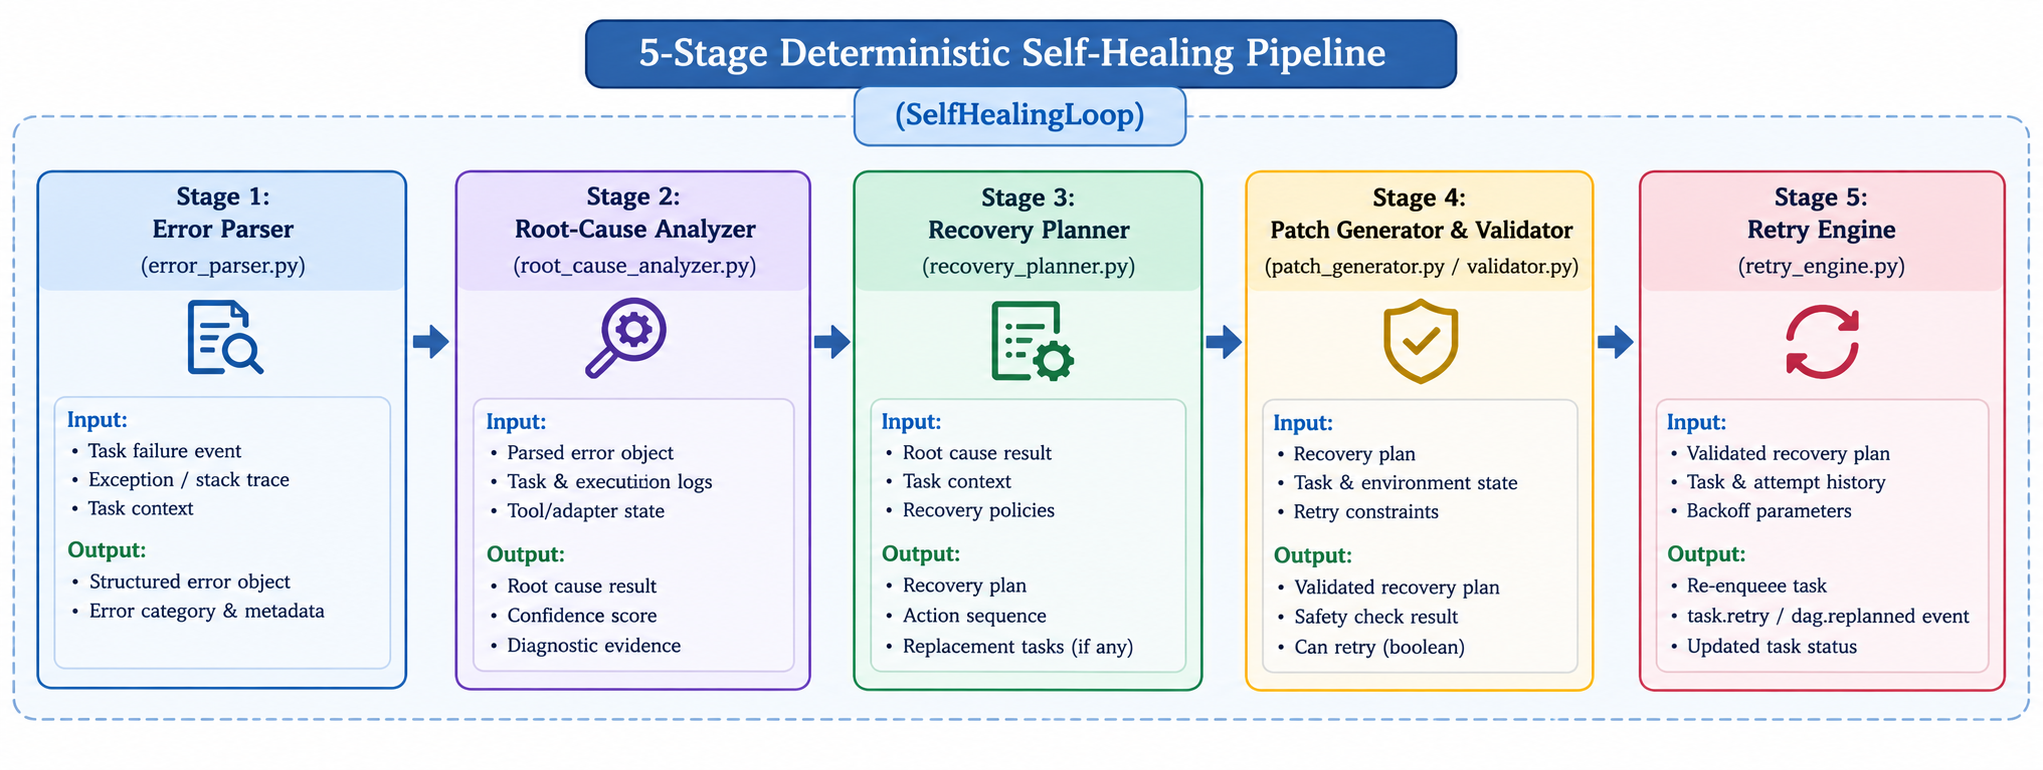
\includegraphics[width=0.95\columnwidth]{extracted_figures/fig_p2__Im1.png}
    \caption{Five-stage deterministic self-healing architecture of Phoenix Agents.}
    \label{fig:architecture}
\end{figure}

The recovery objective function $R(F)$ maps observed faults to either permitted remediation actions or safe terminal rejections:
\begin{equation}
R(F) =
\begin{cases}
A_{\text{retry}}, & \text{if } F \in \mathcal{C}_{\text{recoverable}} \land k_i < K_{\text{max}}, \\
A_{\text{reject}}, & \text{if } F \in \mathcal{C}_{\text{unsafe}} \lor k_i \ge K_{\text{max}}.
\end{cases}
\end{equation}
where $k_i$ is the retry counter for task $v_i$, $K_{\text{max}} = 3$ is the maximum allowed retry budget, $A_{\text{retry}}$ applies deterministic parameter patching or adapter substitution, and $A_{\text{reject}}$ triggers safe failure escalation.

\subsection{Detailed 5-Stage Recovery Pipeline Breakdown}
The self-healing workflow is executed sequentially across five specialized, in-process software modules:

\subsubsection{Stage 1: Error Parser (\texttt{error\_parser.py})}
Intercepts published \texttt{task.failed} event payloads and parses unhandled stack traces into structured error objects, extracting error strings, failing module paths, adapter bindings $\tau_i$, and payload parameters $\theta_i$.

\subsubsection{Stage 2: Root-Cause Analyzer (\texttt{root\_cause\_analyzer.py})}
Evaluates parsed error objects against deterministic rule sets to classify faults into a 5-tier taxonomy:
\begin{equation}
\mathcal{C} \in
\begin{Bmatrix}
\text{Timeout}, & \text{Missing Resource}, \\
\text{Tool/Adapter Failure}, & \text{Invalid Action}, \\
\multicolumn{2}{c}{\text{State Inconsistency}}
\end{Bmatrix}
\end{equation}

\subsubsection{Stage 3: Recovery Planner (\texttt{recovery\_planner.py})}
Evaluates whether the classified fault is recoverable and checks retry budget constraints ($k_i < K_{\text{max}}$). If $k_i \ge K_{\text{max}}$ or if the fault is classified as unsafe (Invalid Action, State Inconsistency), it marks the task as unrecoverable and emits a \texttt{task.rejected} event.

\subsubsection{Stage 4: Patch Generator (\texttt{patch\_generator.py})}
Constructs the required corrective action using the selected deterministic recovery strategy:
\begin{itemize}
    \item \textbf{Exponential Backoff:} Calculates delay $\Delta t = 2^{k_i} \times 1.0\,\text{s}$ for Timeout faults.
    \item \textbf{Parameter Patching:} Corrects missing file paths or parameters in $\theta_i$ by inspecting ancestor task outputs in graph $G$.
    \item \textbf{Adapter Substitution:} Queries \texttt{ToolRegistry} for a functional substitute adapter $\tau'_i$ for Tool/Adapter Failure faults.
    \item \textbf{Topological Replanning:} Prunes invalid downstream subgraphs and synthesizes a replacement graph $G'$ if structural failure occurs.
\end{itemize}

\subsubsection{Stage 5: Retry Engine (\texttt{retry\_engine.py})}
Applies generated patches, increments retry counter $k_i \leftarrow k_i + 1$, resets task status $S_i \leftarrow \text{READY}$, and dispatches a typed \texttt{task.retry} or \texttt{dag.replanned} event over the EventBus.

\begin{table*}[t]
\centering
\caption{\chg{Architectural and Reliability Mechanism Comparison}}
\label{tab:system_comparison}
\footnotesize
\begin{tabularx}{\textwidth}{p{0.16\textwidth}p{0.24\textwidth}p{0.22\textwidth}p{0.18\textwidth}X}
\toprule
\textbf{\chg{Approach}} & \textbf{\chg{Recovery Method}} & \textbf{\chg{Fault Taxonomy / Handling}} & \textbf{\chg{Safety Handling}} & \textbf{\chg{Retry Policy}} \\
\midrule
Babu and Agrawal~\cite{babu2026} & Failure-class mapping with targeted recovery & Tool and orchestration failures & \chg{Silent-failure verification} & \chg{Explicit recovery budget} \\
Jeong and Shin~\cite{jeong2026} & Failure detection, reliability assessment, and self-healing & Hallucination, execution, and reasoning failures & \chg{Failure-aware recovery} & \chg{Re-execution until satisfactory result} \\
Patel et al.~\cite{patel2026b} & Cooperative multi-agent learning & System-level performance and infrastructure failures & \chg{Coordinated corrective actions} & \chg{Learned recovery policy} \\
BacktrackAgent~\cite{wu2025} & Verifier, judger, and reflector modules & GUI action errors and ineffective actions & \chg{Error detection before rewriting} & \chg{Bounded backtracking iterations} \\
\textbf{Phoenix (Proposed)} & \textbf{Five-stage deterministic pipeline} & \textbf{Structured execution-fault taxonomy} & \textbf{\chg{100\% safe rejection}} & \textbf{\chg{Bounded retry ($K_{\text{max}} = 3$)}} \\
\bottomrule
\end{tabularx}
\end{table*}

\section{Methodology and Implementation}
The self-healing architecture of Phoenix Agents is implemented as a modular Python 3.11 package integrated directly within the execution engine kernel.

\subsection{Asynchronous In-Process Event Backbone (EventBus)}
Phoenix Agents uses an in-process asynchronous publish--subscribe EventBus for event delivery, while the five recovery stages execute sequentially within the recovery handler. The EventBus is constructed over Python's native \texttt{asyncio} event loop. Rather than incurring network IPC delays, event objects are published directly to memory channels.

When a tool adapter fails, the Worker Agent publishes a strongly typed \texttt{task.failed} event containing:
\begin{equation}
\text{Payload} = \langle \text{task\_id}, \tau_i, \theta_i, e_{\text{exception}}, \text{traceback\_str} \rangle
\end{equation}
Handler callbacks in the Healing Agent process events asynchronously as non-blocking coroutines without stalling concurrent DAG task branches.

\subsection{Supervisory Contract Verification Engine (SupervisorAgent)}
Before a task is marked as completed, the Supervisor Agent evaluates tool execution artifacts $O_i$ against pre-registered contract assertions:
\begin{equation}
\Psi(v_i, O_i) = (\text{exit\_code} == 0) \land (O_i \models \text{Schema}(v_i)) \land (\text{FileExists}(O_i))
\end{equation}
If any assertion evaluates to false, the Supervisor transitions the node status $S_i \leftarrow \text{FAILED}$ and publishes the failure diagnostic payload to trigger self-healing.

\subsection{Fault Taxonomy \& Pattern Matching Classifier (\texttt{root\_cause\_analyzer.py})}
\chg{The Root-Cause Analyzer processes exception strings using deterministic rule matching across a 5-tier taxonomy: recoverable faults comprise \textit{Timeout} (mitigated via bounded retry with exponential backoff), \textit{Missing Resource} (parameter/path correction from ancestor task outputs), and \textit{Tool/Adapter Failure} (adapter substitution via \texttt{ToolRegistry}); unsafe faults comprise \textit{Invalid Action} and \textit{State Inconsistency}, both mapped to immediate safe rejection and failure escalation.}

\subsection{Parameter Patching \& Dynamic Adapter Resolution (\texttt{patch\_generator.py})}
\begin{itemize}
    \item \textbf{Parameter Patching:} For Missing Resource faults, the Patch Generator inspects ancestor node output dictionaries in graph $G$ to resolve valid target file paths or parameters.
    \item \textbf{Adapter Substitution:} For Tool/Adapter Failure faults, the component queries the central \texttt{ToolRegistry} to resolve a functional substitute adapter $\tau'_i$ capable of executing the intended action.
\end{itemize}

\subsection{Dynamic Topological DAG Replanning (\texttt{orchestrator.py})}
When structural graph breakage occurs (e.g., an unrecoverable failure in a critical dependency node), the Healing Agent invokes dynamic replanning. It prunes invalid downstream subgraphs, updates execution dependencies using Kahn's topological sorting algorithm, and publishes a \texttt{dag.replanned} event to resume graph processing without restarting the entire workflow. The topological replanning capability is part of the implemented recovery architecture but was not included in the 125-trial fault-injection evaluation reported in this paper.

\section{Evaluation Metrics \& Formulas}
To rigorously quantify the resilience, handling overhead, and execution safety of the self-healing subsystem in Phoenix Agents, five primary evaluation metrics are defined:

\subsection{Overall Recovery Ratio ($SR$)}
Measures the overall proportion of all injected fault trials ($N_{\text{injected}} = 125$) resulting in successful automatic recovery:
\begin{equation}
SR = \frac{N_{\text{recovered}}}{N_{\text{injected}}} \times 100
\end{equation}
\textit{Observed Value:} $SR = \frac{75}{125} \times 100 = 60.0\%$ \chg{(Wilson 95\% confidence interval: 51.2\% to 68.2\%; reflects the denominator including 50 intentional safety rejections).}

\subsection{Recoverable-Case Success Rate ($SR_{\text{rec}}$)}
Measures the recovery success rate evaluated strictly across supported recoverable fault classes (Missing Resource, Timeout, Tool/Adapter Failure, where $N_{\text{injected,rec}} = 75$):
\begin{equation}
SR_{\text{rec}} = \frac{N_{\text{recovered,rec}}}{N_{\text{injected,rec}}} \times 100 = \frac{75}{75} \times 100 = 100.0\%
\end{equation}
\textit{Observed Value:} $SR_{\text{rec}} = 100.0\%$ \chg{(Wilson 95\% confidence interval: 95.1\% to 100.0\%)} across all 75 recoverable trials.

\subsection{Safe Rejection Rate ($SR_{\text{safe}}$)}
Measures the proportion of unsafe/unrecoverable fault trials (Invalid Action, State Inconsistency, where $N_{\text{injected,unsafe}} = 50$) correctly identified and blocked by safety guards without initiating unauthorized retries:
\begin{equation}
SR_{\text{safe}} = \frac{N_{\text{rejected,unsafe}}}{N_{\text{injected,unsafe}}} \times 100 = \frac{50}{50} \times 100 = 100.0\%
\end{equation}
\textit{Observed Value:} $SR_{\text{safe}} = 100.0\%$ \chg{(Wilson 95\% confidence interval: 92.9\% to 100.0\%)} across all 50 unsafe trials.

\chg{These 50 evaluated unsafe trials specifically belong to the two unrecoverable classes the rule set was calibrated for (\textit{Invalid Action} and \textit{State Inconsistency}). In the underlying implementation (\texttt{root\_cause\_analyzer.py} and \texttt{recovery\_planner.py}), if an incoming exception does not match any known diagnostic pattern, \texttt{\_synthesize\_diagnosis()} assigns it to \texttt{UNKNOWN\_ROOT\_CAUSE} with confidence score $\le 0.30$; \texttt{RecoveryPlanner.plan()} intercepts this condition (or unhandled exceptions with \texttt{is\_retryable=False}) and immediately issues a non-viable plan (\texttt{NO\_VIABLE\_RECOVERY}), triggering safe failure escalation without retrying. Conversely, if an unsafe fault falsely matches a recoverable rule template, the engine executes bounded retries up to $K_{\text{max}} = 3$; upon each retry, the Supervisor evaluates contract assertions $\Psi(v_i, O_i)$, which continue to fail, leading to budget exhaustion and safe escalation without non-terminating loops.}

\subsection{Software-Level Recovery Handling Latency ($T_R$)}
Measures the in-process execution time required for the 5-stage pipeline to parse the error, classify root causes, patch parameters, and re-enqueue the task: Recovery latency therefore covers the in-process recovery path from fault handling through task re-enqueue.
\begin{equation}
T_R = T_{\text{success}} - T_{\text{fault}}
\end{equation}
\textit{Observed Values:}
\begin{itemize}
    \item Mean $T_R$: 1.30~ms
    \item Median $T_R$: 1.10~ms
    \item Observed Range: 0.51~ms--4.58~ms
\end{itemize}

\subsection{Self-Healing Overhead ($\Delta T_{\text{overhead}}$)}
Measures the extra software-level handling overhead of executing deterministic recovery relative to the fail-fast no-recovery baseline ($T_{\text{no\_rec}}$):
\begin{equation}
\Delta T_{\text{overhead}} = T_{\text{rec}} - T_{\text{no\_rec}} = 1.88\,\text{ms} - 0.44\,\text{ms} = 1.44\,\text{ms}
\end{equation}
\textit{Observed Value:} The system records a measured 1.44~ms of software-level handling overhead relative to the fail-fast baseline.

The values reported for prior approaches were obtained under their respective evaluation protocols and are included for contextual comparison rather than as a controlled head-to-head benchmark.

\begin{table*}[t]
\centering
\caption{Quantitative Performance Comparison Using Reported Metrics}
\label{tab:performance_comparison}
\footnotesize
\begin{tabularx}{\textwidth}{p{0.22\textwidth}p{0.20\textwidth}p{0.14\textwidth}p{0.24\textwidth}X}
\toprule
\textbf{Approach} & \textbf{Success Metric} & \textbf{Reported Value} & \textbf{Evaluation Scale} & \textbf{Recovery-Time Metric} \\
\midrule
\multicolumn{5}{l}{\chg{\textit{Metric definitions: Task success rate: percentage of complete tasks successfully executed; Error recovery accuracy: proportion of errors corrected;}}} \\
\multicolumn{5}{l}{\chg{\textit{Recoverable-case success rate: recovery rate on supported recoverable faults; Recovery time per step: mean latency required for recovery handling per step.}}} \\
\midrule
Babu and Agrawal~\cite{babu2026} & Task success rate & 98.8\% & 100-task fault-injection benchmark & Recovery time not reported \\
BacktrackAgent--Mobile3M~\cite{wu2025} & Error recovery accuracy & 38.93\% & Mobile3M GUI evaluation & 1.938~s per step \\
BacktrackAgent--Auto-UI~\cite{wu2025} & Error recovery accuracy & 31.24\% & Auto-UI GUI evaluation & 1.374~s per step \\
Patel et al.~\cite{patel2026b} & Recovery-time reduction & Up to 47\% & Simulated and real-world failure scenarios & Recovery time reduced by up to 47\% \\
\textbf{Phoenix (Proposed)} & \textbf{Recoverable-case success rate} & \textbf{100.0\%} & \textbf{125 controlled trials} & \textbf{1.30~ms mean} \\
\bottomrule
\multicolumn{5}{p{\textwidth}}{\chg{\textsuperscript{*}Note: Prior values are as reported under their respective evaluation protocols and benchmarks, providing contextual reference rather than a direct head-to-head comparison.}}
\end{tabularx}
\end{table*}

\subsection{Operational Discussion}
The evaluation results indicate that the recovery subsystem provides a bounded execution-level mechanism for handling failures without extending the active reasoning loop with additional model inference. The separation between fault detection, classification, remediation, and verification allows each recovery action to remain associated with an explicit fault category and a corresponding deterministic strategy. This structure also makes the recovery path observable at the supervisor level, which supports measurement of both successful remediation and safe rejection outcomes.

A practical implication of the architecture is that recoverable and unsafe failures are treated differently rather than forcing every detected exception through the same retry path. Parameter and adapter faults can be repaired through bounded transformations, while faults that cannot be safely remediated are rejected according to the supervisor contract. The experimental results therefore evaluate not only successful recovery but also the system's ability to terminate unsafe cases without falsely reporting completion.

The measured recovery latency further indicates that the self-healing logic adds a small software-level handling cost relative to the overall automation workflow. Because the recovery pipeline is deterministic and bounded, its behavior can be reproduced under the same injected fault conditions. This provides a concrete basis for extending the evaluation to larger workflow graphs, additional desktop and browser failure modes, and more complex state-reconstruction scenarios while preserving the same recovery and safety contracts.

\section{Conclusion and Future Work}

\subsection{Conclusion}
This paper presented the bounded self-healing subsystem of Phoenix Agents, a deterministic, LLM-free recovery framework for multi-agent desktop automation. By isolating error diagnosis, root-cause classification, strategy selection, patch generation, and retry execution into an in-process 5-stage pipeline, the system remediates execution exceptions without invoking active LLM inferencing during the error mitigation loop.

Key experimental findings demonstrate:
\begin{enumerate}
    \item \textbf{Millisecond-Scale Recovery Handling:} The 5-stage pipeline achieves a mean software-level recovery latency of 1.30~ms (median 1.10~ms), with a measured 1.44~ms of software-level handling overhead relative to the fail-fast baseline.
    \item \textbf{\chg{Fault Recovery and Safe Rejection:}} \chg{Across 125 controlled fault-injection trials, the pipeline recovered all 75 faults in the three recoverable classes (Missing Resource, Timeout, Tool/Adapter Failure; 75/75) and rejected all 50 faults in the two unsafe classes (Invalid Action, State Inconsistency; 50/50), giving 60.0\% overall recovery (75/125) when counting safe rejections as unrecovered rather than a failure to heal recoverable faults.}
    \item \textbf{100\% Safe Rejection Rate:} Across 50 unsafe fault trials (Invalid Action, State Inconsistency), safety guards correctly detected and rejected all unsafe operations (50/50), preventing uncontrolled retries.
    \item \textbf{Recovery vs.\ No-Recovery Comparison:} Controlled comparisons between recovery-enabled and recovery-disabled configurations established a 100\% workflow completion rate with deterministic recovery enabled versus 0\% with recovery disabled under transient error workloads.
\end{enumerate}

\subsection{Future Work}
Future research will expand the self-healing subsystem of Phoenix Agents along three primary dimensions:
\begin{itemize}
    \item \textbf{Real Browser \& Operating System Chaos Testing:} Transitioning from synthetic software-level fault injection to live browser and desktop chaos testing, evaluating recovery under dynamic DOM locator shifts, network latency spikes, and OS process crashes.
    \item \textbf{Safe Checkpoint Rollback \& State Reconstruction:} Developing transactional checkpointing mechanisms to enable safe state rollback and graph reconstruction when encountering complex workflow state inconsistencies.
    \item \textbf{Large-Scale Scalability Profiling:} Evaluating recovery handling overhead and concurrency limits as the number of simultaneous multi-agent workflows scales across multi-node execution clusters.
\end{itemize}

\begin{thebibliography}{12}

\bibitem{babu2026}
R.~S.~Babu and A.~Agrawal, ``Self-Healing Agentic Orchestrators for Reliable Tool-Augmented Large Language Model Systems,'' \chg{\url{https://arxiv.org/abs/2606.01416}}, 2026.

\bibitem{jeong2026}
C.~Jeong and Y.~Shin, ``A Self-Healing Framework for Reliable LLM-Based Autonomous Agents,'' \chg{\url{https://arxiv.org/abs/2605.06737}}, 2026.

\bibitem{guo2026}
X.~Guo et al., ``EvoConfig: Self-Evolving Multi-Agent Systems for Efficient Autonomous Environment Configuration,'' \chg{\url{https://arxiv.org/abs/2601.16489}}, 2026.

\bibitem{ju2025}
T.~Ju et al., ``When Disagreements Elicit Robustness: Investigating Self-Repair Capabilities under LLM Multi-Agent Disagreements,'' \chg{\url{https://arxiv.org/abs/2502.15153}}, 2025.

\bibitem{bara2026}
A.~Bara, G.~Dobri\c{t}a, and S.-V.~Oprea, ``Think it, Run it: Autonomous machine learning pipeline generation via self-healing multi-agent artificial intelligence,'' \emph{Knowledge-Based Systems}, vol. 351, p. 116688, 2026, \chg{\url{https://doi.org/10.1016/j.knosys.2026.116688}}.

\bibitem{wang2026}
F.~Wang et al., ``Detecting and Repairing Role Drift in Multi-Agent Collaboration with Lightweight Protocols,'' in \emph{Proc. CNML}, 2026, \chg{\url{https://doi.org/10.1109/CNML68938.2026.11453032}}.

\bibitem{patel2026a}
T.~P.~Patel et al., ``Predictive Self-Healing for Multi-Agent LLM Pipelines Using Model Predictive Control,'' in \emph{Proc. IEEE SusTech}, 2026, \chg{\url{https://doi.org/10.1109/SUSTECH67720.2026.11536606}}.

\bibitem{patel2026b}
T.~P.~Patel et al., ``Self-Healing AI Systems using Multi-Agent Learning,'' in \emph{Proc. ISIBER}, 2026, \chg{\url{https://doi.org/10.1109/ISIBER68248.2026.11470173}}.

\bibitem{garcia2026}
B.~Garc\'{\i}a et al., ``A survey on Selenium usage, practices, and challenges in end-to-end testing,'' \emph{Information and Software Technology}, vol. 194, p. 108077, 2026, \chg{\url{https://doi.org/10.1016/j.infsof.2026.108077}}.

\bibitem{nguyen2025}
D.~Nguyen et al., ``GUI Agents: A Survey,'' in \emph{Findings of ACL}, pp. 22522--22538, 2025, \chg{\url{https://aclanthology.org/2025.findings-acl.1150/}}.

\bibitem{bajoria2026}
S.~Bajoria et al., ``From Language Models to Agentic AI: A Survey of Autonomous, Action-Enabled, and Collaborative LLM Agents,'' \emph{Cognitive Computation}, vol. 18, p. 103, 2026, \chg{\url{https://doi.org/10.1007/s12559-026-10368-2}}.

\bibitem{wu2025}
Q.~Wu, P.~Gao, W.~Liu, and J.~Luan, ``BacktrackAgent: Enhancing GUI Agent with Error Detection and Backtracking Mechanism,'' in \emph{Proc. Conference on Empirical Methods in Natural Language Processing (EMNLP)}, pp. 4250--4272, 2025, \chg{\url{https://aclanthology.org/2025.emnlp-main.245/}}.

\end{thebibliography}

\end{document}
